\documentclass[tikz,border=10pt]{standalone}
\usetikzlibrary{angles,quotes}
\begin{document}
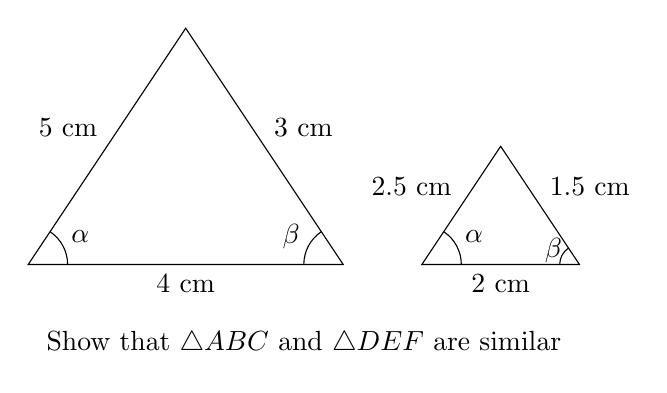
\begin{tikzpicture}
  % Define the vertices of the triangles
  \coordinate (A) at (0,0);
  \coordinate (B) at (4,0);
  \coordinate (C) at (2,3);
  \coordinate (D) at (5,0);
  \coordinate (E) at (7,0);
  \coordinate (F) at (6,1.5);

  % Draw the triangles
  \draw (A) -- node[below]{4 cm} (B) -- node[above right]{3 cm} (C) -- node[above left]{5 cm} cycle;
  \draw (D) -- node[below]{2 cm} (E) -- node[above right]{1.5 cm} (F) -- node[above left]{2.5 cm} cycle;

  % Label angles
  \pic [draw, -, angle radius=0.5cm, "$\alpha$", angle eccentricity=1.5] {angle=B--A--C};
  \pic [draw, -, angle radius=0.5cm, "$\alpha$", angle eccentricity=1.5] {angle=E--D--F};
  \pic [draw, -, angle radius=0.5cm, "$\beta$", angle eccentricity=1.5] {angle=C--B--A};
  \pic [draw, -, angle radius=0.25cm, "$\beta$", angle eccentricity=1.5] {angle=F--E--D};

  % Question text
  \node at (3.5,-1) {Show that $\triangle ABC$ and $\triangle DEF$ are similar};
\end{tikzpicture}
\end{document}